%% 
%% Template article for Environmental Modeling and Software using Elsevier's document class `elsarticle'
%% with numbered style bibliographic references
%%
\documentclass[final,3p,times]{elsarticle}

%% Use the option review to obtain double line spacing
%% \documentclass[preprint,review,12pt]{elsarticle}

%% For final submission:
%% \documentclass[final,3p,times]{elsarticle}

%% The amssymb package provides various useful mathematical symbols
\usepackage{amssymb}
%% The amsmath package provides various useful equation environments
\usepackage{amsmath}
%% The amsthm package provides extended theorem environments
\usepackage{amsthm}
%% The lineno packages adds line numbers
\usepackage{lineno}
\usepackage{graphicx}
\usepackage{hyperref}
\usepackage{booktabs}
\usepackage{float}
\usepackage{url}

\journal{Environmental Modeling and Software}

\begin{document}

\begin{frontmatter}

%% Title, authors and addresses
\title{SWATGenX: An automated Web application platform for generating SWAT+ with NHDPlus HR across CONUS}

\author[1]{Vahid Rafiei}
\author[1]{A. Pouyan Nejadhashemi\corref{cor1}}
\cortext[cor1]{Corresponding author. Tel.: +1 (517) 432-7653. Email: pouyan@msu.edu}
\ead{pouyan@msu.edu}
\address[1]{Department of Biosystems and Agricultural Engineering, Michigan State University (MSU), USA}

\begin{abstract}
% An overview of the work, aim, objectives, methods and product
% Abstract should be approximately 250 words
\end{abstract}

\begin{keyword}
SWAT+ \sep groundwater modeling \sep hydrological models \sep CONUS \sep web application \sep NHDPlus HR
\end{keyword}

\end{frontmatter}

%% Uncomment to enable line numbers
%% \linenumbers

\section{Introduction}
\label{sec:introduction}

Regional hydrological modeling is crucial for evaluating impacts of natural and human-induced changes on water resources. Such models guide flood control, water supply planning, and ecosystem conservation decisions, providing actionable information for sustainable water resource management. In agricultural landscapes, hydrological models optimize irrigation scheduling, estimate crop water requirements, and assess how farming practices affect water availability and quality. By improving agricultural water-use efficiency, these models bridge environmental and agricultural research, informing science-based land and water management decisions across scales -- from farm fields to regional watersheds.

Building and deploying hydrological models at large scales presents several challenges. Data acquisition and integration is a significant hurdle: comprehensive models require merging disparate data sources (hydrography, climate, land cover, soils), which is labor-intensive and technically complex. Even with unprecedented detail from recent geospatial datasets -- such as the NHDPlus High Resolution dataset (NHDPlus HR) providing a $\sim$1:24,000-scale hydrographic network with approximately 27 million stream reaches across the contiguous U.S. -- assembling and processing these massive datasets into a modeling framework remains non-trivial. Computational constraints further limit widespread modeling: large-scale watershed simulations require significant memory and processing power, often necessitating high-performance computing resources.

These constraints are evident in existing national-scale modeling efforts. The National Agroecosystem Model (NAM) and the USGS National Hydrologic Model (NHM) have relied on moderate-resolution hydrographic data (1:100,000-scale NHD dataset) when simulating across the entire country. The 1:100k stream network contains roughly 2.5 million river reaches, an order of magnitude fewer than NHDPlus HR's $\sim$27 million reaches. Such coarse representation simplifies river connectivity and basin detail, leading to missed small-scale features, limited local relevance, and reduced stakeholder confidence. Similarly, Princeton's HydroGEN project highlights the immense data-handling and computational burden involved in scaling up hydrologic models, even with modern cloud infrastructure.

We developed a scalable, automated platform (SWATGenX) for high-resolution watershed modeling to address these limitations. The system utilizes modern data streams and computing approaches, effectively bridging detailed data and user-friendly model generation. SWATGenX builds a SWAT+ hydrological model for any given watershed outlet, harnessing NHDPlus HR for delineating streams and subbasins, ensuring even small tributaries, headwater catchments, and water bodies are represented. The platform integrates complementary high-resolution datasets seamlessly, including gridded climate inputs (PRISM, LOCA2), the National Solar Radiation Database, and land use/soil data. The entire workflow is orchestrated through a hierarchical database and APIs that connect to national data services, including the USGS National Water Information System (NWIS) to obtain observed streamflow and basin characteristics for over 36,000 gauging stations across the United States.

This work introduces our novel platform with several key contributions: (1) High-resolution model generation at scale, constructing coupled groundwater--surface water models using fine-resolution hydrographic data with an efficient online platform allowing users to generate calibrated SWAT+ models on demand; (2) Integration of groundwater and surface water through the SWAT+ gwflow module, demonstrated through 58 paired models in Michigan's Lower Peninsula to evaluate improvements gained by coupling groundwater flow; and (3) Regional application and evaluation across the Michigan Lower Peninsula, calibrating and validating models against observed streamflow to assess accuracy and identify systematic biases. By significantly reducing barriers to high-resolution hydrological modeling, our framework enables more accessible and data-rich models that support better environmental and agricultural decision-making across the United States.

\section{Materials and Methods}
\label{sec:methods}

\subsection{Overview of the SWATGenX system}
\label{subsec:system_overview}

SWATGenX is a scalable, automated platform designed to generate high-resolution SWAT+ models across the Conterminous United States (CONUS). The system leverages national datasets, particularly the NHDPlus High Resolution (HR) which provides a 1:24,000-scale hydrographic network with approximately 27 million identifiable channels across CONUS. This level of detail represents a significant improvement over previous modeling frameworks that relied on the 1:100,000-scale NHD dataset, which only contains about 2.5 million river reaches.

At its core, SWATGenX is a Python-based program module that automates the entire workflow of hydrological model creation. The system architecture consists of three main components: (1) a data processing pipeline for acquiring and preprocessing geospatial and hydrological data, (2) a model generation engine that processes these data into SWAT+ model structures, and (3) an application programming interface (API) that connects to various national data services.

The data processing pipeline begins by extracting hydrographical data from the NHDPlus HR database, including streams (NHDFlowline), drainage areas (NHDPlusCatchment), waterbodies (NHDWaterbody), and value-added attributes (NHDPlusFlowlineVAA). These data undergo rigorous preprocessing to ensure consistency, including coordinate system projection, removal of divergence issues, resolution of lake-stream connections, and enforcement of the "one-outlet rule" for each subbasin.

The model generation engine integrates QSWAT+ and SWAT+Editor APIs to automatically construct the SWAT+ project structure. This component handles the creation of Hydrologic Response Units (HRUs), channel routing structures, and waterbody connections. For groundwater integration, the system incorporates the SWAT+ gwflow module, which simulates groundwater flow and groundwater-surface water interactions at 250m resolution.

The API component connects SWATGenX to multiple national data services, including the USGS National Water Information System (NWIS) for streamflow data from over 36,000 stations, PRISM for climate data at 4km resolution, and the National Solar Radiation Database (NSRDB) for energy balance parameters. This integration allows for seamless data extraction and processing, enabling users to generate complete SWAT+ models with minimal input.

The entire process is highly efficient, with model generation taking between 20 seconds for small watersheds to just a few minutes for larger basins. This efficiency, combined with the system's ability to handle high-resolution data, makes SWATGenX a powerful tool for watershed modeling at scales ranging from individual HUC12 watersheds to regional or national applications.

Figure \ref{fig:workflow} illustrates the automated workflow of SWATGenX, showing the data acquisition, processing, and model generation pipeline.

\begin{figure}[htbp]
    \centering
    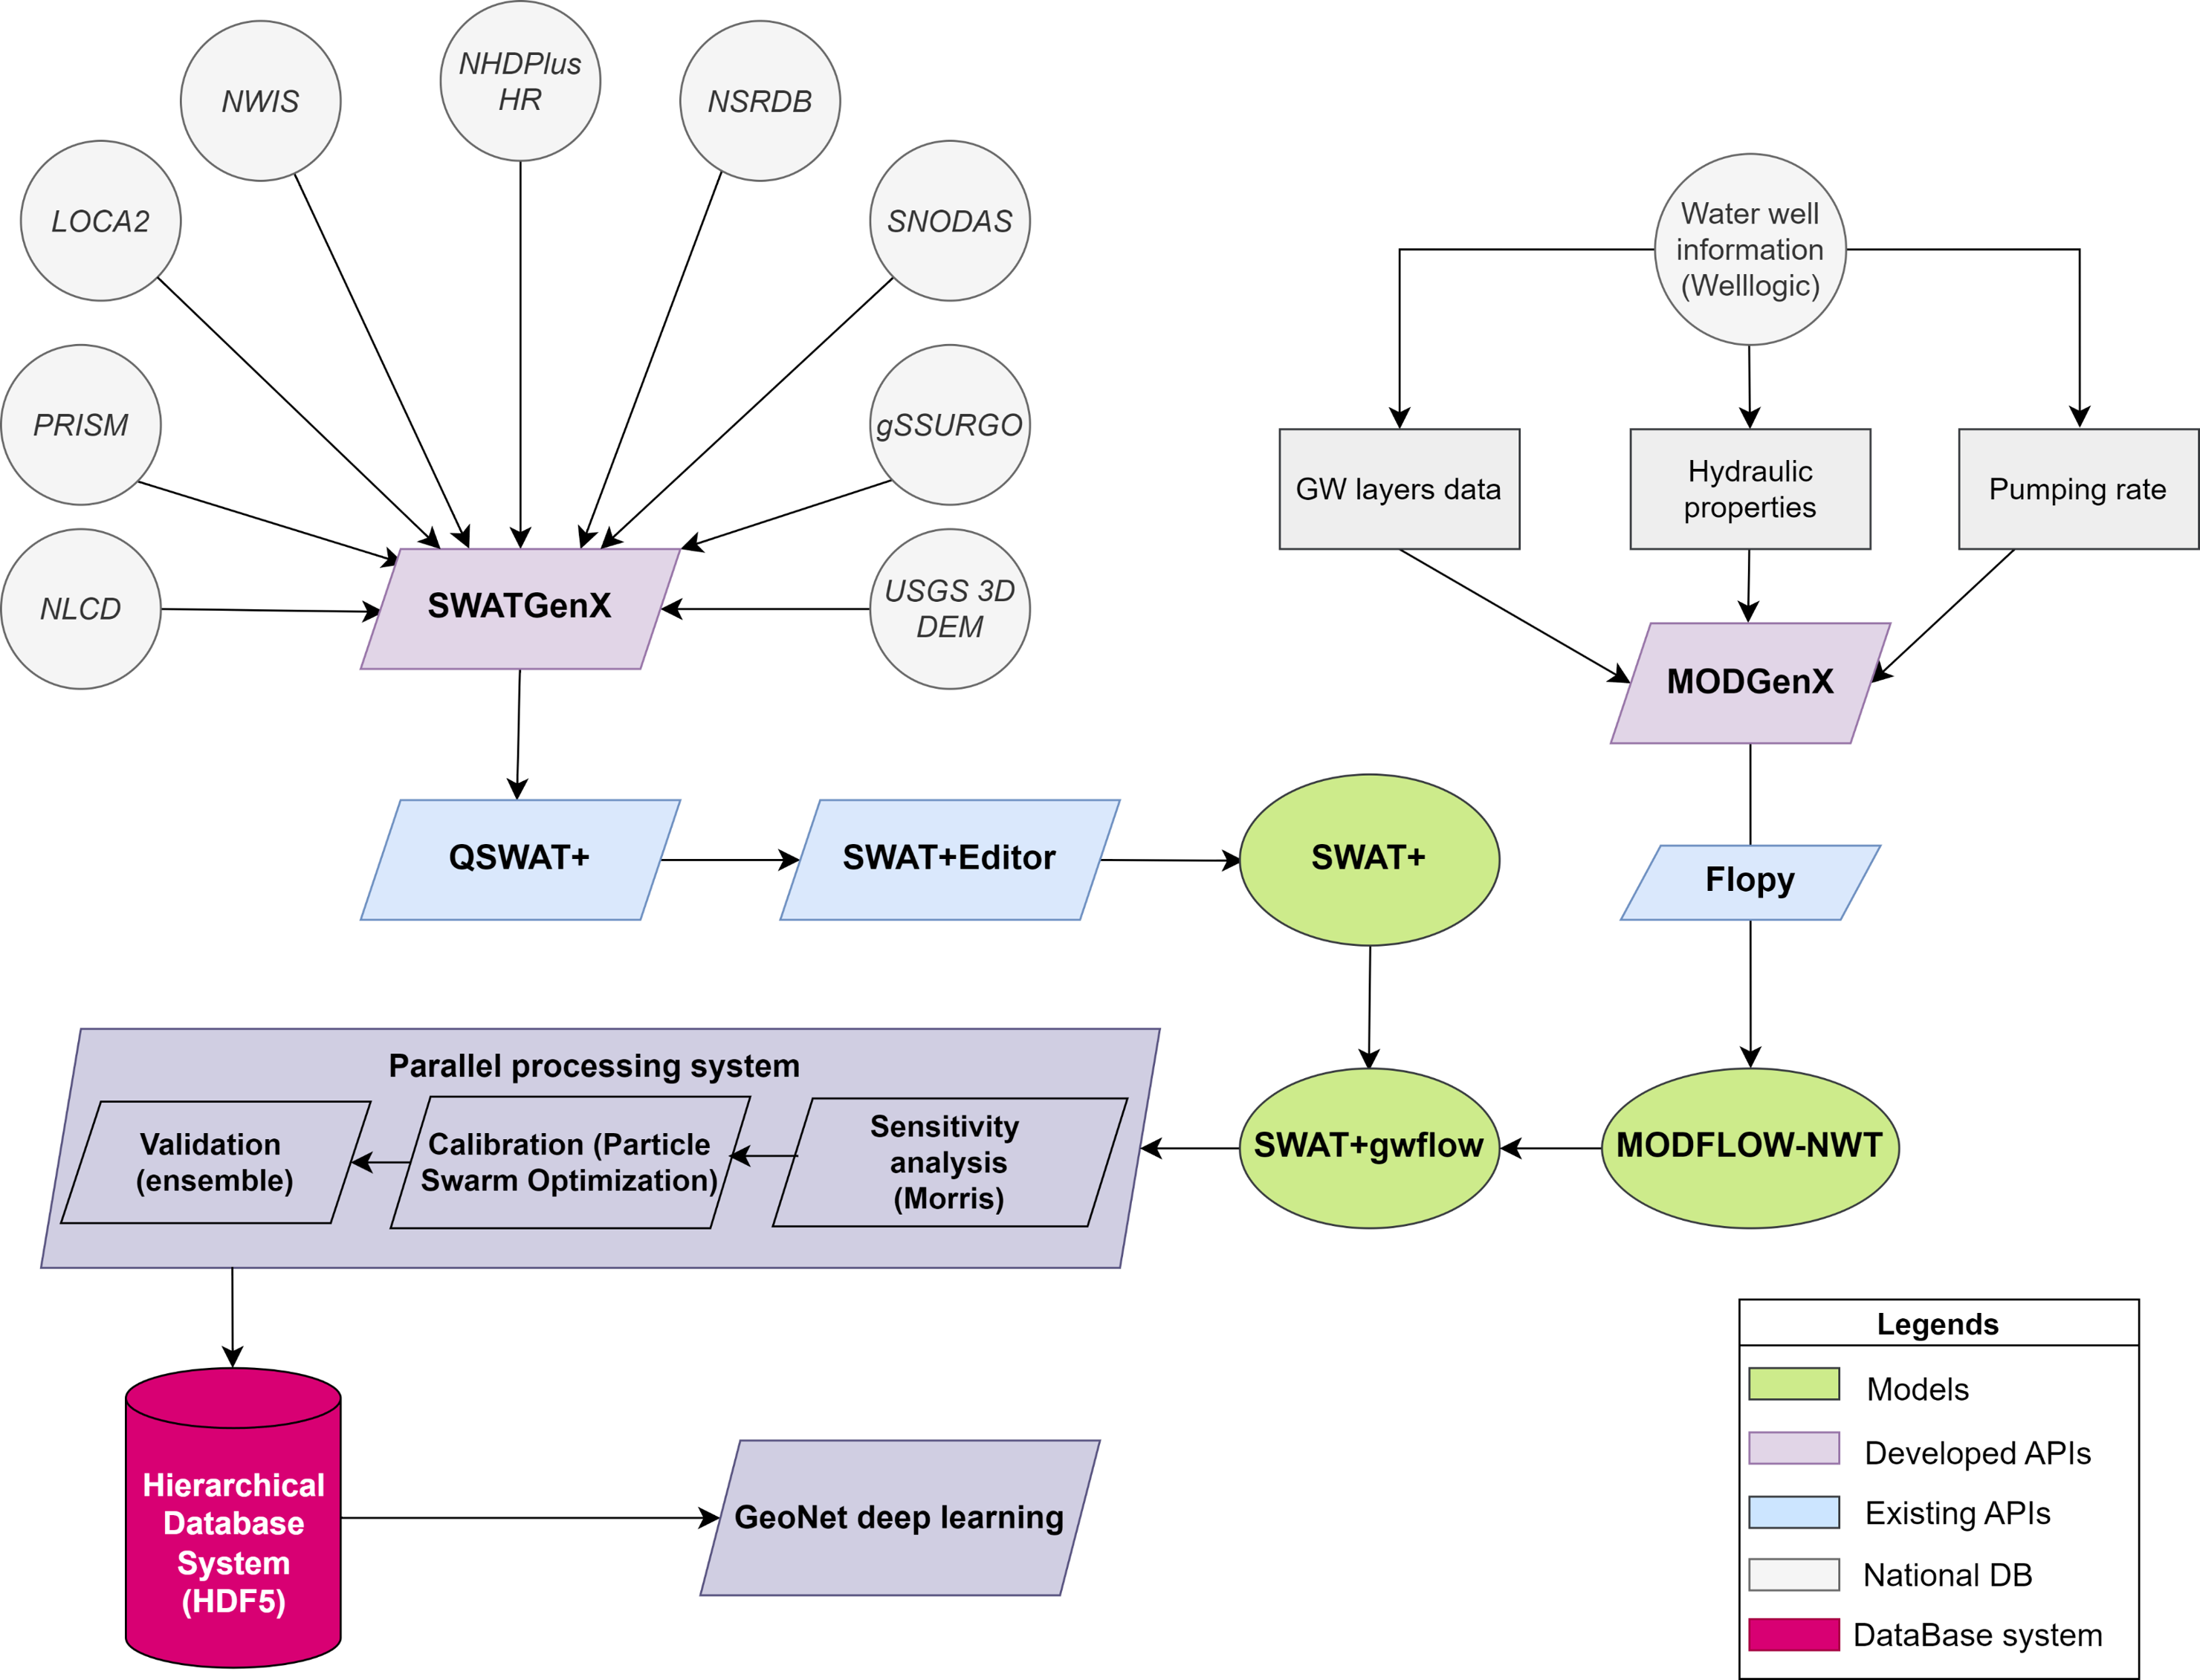
\includegraphics[width=\textwidth]{/data/SWATGenXApp/codes/docs/figures/SWATGenX.png}
    \caption{Flowchart of the SWATGenX automated workflow for SWAT+ model generation, showing data acquisition, processing, and model preparation steps.}
    \label{fig:workflow}
\end{figure}

\subsection{Data sources}
\label{subsec:data_sources}

Table \ref{tab:data_sources} summarizes the key datasets integrated into the SWATGenX platform. These diverse data sources are automatically acquired, processed, and integrated to generate consistent, high-resolution SWAT+ models. The system handles coordinate system transformations, temporal alignments, and spatial interpolations required to harmonize these heterogeneous datasets into a coherent modeling framework.

\begin{table}[htbp]
\centering
\caption{Data sources used in the SWATGenX platform.}
\label{tab:data_sources}
\begin{tabular}{p{3.5cm}p{2cm}p{2.5cm}p{6.5cm}}
\hline
\textbf{Dataset Name} & \textbf{Resolution} & \textbf{Type} & \textbf{Details} \\
\hline
NHDPlus High Resolution (HR) & 1:24,000-scale & Hydrography & Comprehensive stream network with ~27 million reaches across CONUS, including flowlines, catchments, waterbodies, and value-added attributes \\
\hline
Watershed Boundary Dataset (WBD) & 1:24,000-scale & Watershed delineation & HUC8 and HUC12 watershed boundaries used as context for model development \\
\hline
PRISM Climate Data & 4 km & Meteorological & Daily precipitation, temperature (min/max), and other climate variables from 1981 to present \\
\hline
National Solar Radiation Database (NSRDB) & 4 km & Meteorological & Solar radiation, wind speed, and relative humidity data for energy balance calculations \\
\hline
LOCA2 Climate Projections & Various (typically 6 km) & Climate projections & Downscaled climate projections from global climate models \\
\hline
National Land Cover Database (NLCD) & 30 m & Land use/land cover & 16 major land cover classes including various forest types, agricultural land, urban areas, and wetlands \\
\hline
SSURGO Soil Database & 1:24,000-scale & Soils & Detailed soil properties for modeling infiltration, soil water movement, and nutrient cycling \\
\hline
STATSGO Soil Database & 1:250,000-scale & Soils & State-level soil data used where SSURGO is unavailable \\
\hline
USGS National Water Information System (NWIS) & Point data & Streamflow & Records for over 36,000 gauging stations with daily and sub-daily time steps \\
\hline
Wellogic Groundwater Database & Point data & Groundwater & Over 600,000 well records with lithological data including aquifer thickness, hydraulic conductivity, static water level, and transmissivity \\
\hline
\end{tabular}
\end{table}

\subsection{SWATGenX implementation using national datasets}
\label{subsec:implementation}

SWATGenX implements a systematic workflow for transforming national geospatial datasets into ready-to-use SWAT+ hydrological models. This implementation follows a modular framework organized around key hydrological processes and data types, with seamless integration between components. Figure \ref{fig:workflow} illustrates this workflow, highlighting how different data streams converge to create comprehensive watershed models.

\subsubsection{Watershed Delineation Process}
The foundation of model generation begins with hydrographic data processing. Using NHDPlus HR as the base dataset, SWATGenX extracts watershed boundaries, stream networks, and their attributes for a user-specified outlet point (typically a USGS gauging station). The system employs a hierarchical approach based on Vector Processing Unit Identifiers (VPUIDs) from NHDPlus HR, allowing efficient handling of regional data.

A critical challenge in adapting NHDPlus HR data for SWAT+ involves addressing subbasin delineation issues, particularly the requirement that each subbasin must have exactly one outlet. The system automatically detects and resolves cases of multiple outlets through an iterative tracing algorithm that splits problematic subbasins while maintaining hydrological connectivity. Similarly, the system handles lake-stream connections by identifying inflows and outflows, resolving complex lake networks, and ensuring proper routing through water bodies.

\subsubsection{Environmental Data Processing}
Once the watershed structure is established, SWATGenX integrates multiple environmental datasets to characterize the watershed's physical properties:

\begin{itemize}
    \item \textbf{Climate data integration}: The system processes PRISM data to establish weather stations on a 4km grid covering the watershed. For each station, daily precipitation and temperature time series are extracted and formatted for SWAT+. To complete the energy balance requirements, the system extracts solar radiation, wind speed, and relative humidity from the National Solar Radiation Database, applying elevation corrections when necessary.
    
    \item \textbf{Land surface characterization}: Land use classifications from the National Land Cover Database are processed to define spatial patterns of vegetation, urban areas, and other land cover types. Soil properties from SSURGO/STATSGO databases are extracted and reclassified to SWAT+ soil parameters. Digital Elevation Model data provides the topographic context for the watershed.
\end{itemize}

These environmental layers are spatially aligned with the hydrographic framework, ensuring consistent geospatial representation throughout the model.

\subsubsection{Model Assembly and Validation}
In the final stage, SWATGenX assembles the processed data into a complete SWAT+ model structure. This involves:

\begin{enumerate}
    \item Creating spatial input files (rasters and shapefiles) conforming to SWAT+ requirements
    \item Automatically generating Hydrologic Response Units (HRUs) by overlaying land use, soil, and slope data
    \item Establishing channel routing parameters based on NHDPlus HR attributes
    \item Configuring management operations based on land use types
    \item Integrating USGS streamflow observation data at appropriate locations for model calibration
\end{enumerate}

The system leverages the QSWAT+ interface and SWAT+ Editor to create the model database and input files without manual intervention. A validation run ensures the model executes successfully before delivery to the user.

\subsubsection{Integration Efficiency}
A key innovation in SWATGenX is its seamless integration of disparate data sources and processes. The system maintains a consistent spatial reference framework throughout, automatically handling coordinate transformations and resolution differences between datasets. This integration reduces what traditionally requires weeks of manual data preparation and model setup to an automated process completed in minutes.

The implementation incorporates extensive quality assurance checks, including topological validation of stream networks, verification of water balance in subbasins, and consistency checks for climate station coverage. These checks ensure the resulting SWAT+ models are not only quick to generate but also scientifically sound and ready for calibration.

By abstracting the technical complexities of model setup, SWATGenX makes high-resolution hydrological modeling more accessible to researchers, watershed managers, and policymakers who may lack specialized GIS expertise but need robust modeling tools for decision support.

\subsection{Groundwater modeling implementation and integration}
\label{subsec:groundwater}

The SWATGenX platform implements groundwater processes through two complementary approaches: (1) integration of the SWAT+ gwflow module for coupled surface-groundwater simulations, and (2) development of standalone MODFLOW models using a custom MODGenX framework. This dual approach allows us to balance computational efficiency with physical process representation.

\subsubsection{SWAT+ gwflow Module Implementation}
For integrated surface-groundwater modeling, we implemented the recently developed gwflow module within SWAT+. This module represents a significant advancement over the original SWAT+ groundwater representation, providing a physically-based, spatially-distributed simulation of groundwater processes. The gwflow module:

\begin{itemize}
    \item Implements a finite difference grid (250m resolution) within each subbasin
    \item Simulates lateral groundwater flow based on Darcy's law
    \item Models groundwater-surface water interactions at rivers and lakes
    \item Accounts for recharge from the soil profile and discharge to streams
\end{itemize}

A key challenge in implementing gwflow is parameterizing the groundwater hydraulic properties across large domains. For the Michigan case study, we leveraged the Wellogic database containing over 600,000 water well records with lithological information. Using Empirical Bayesian Kriging (EBK), we developed consistent datasets for hydraulic conductivity, groundwater head, transmissivity, and aquifer depth across the state. The resulting groundwater properties were aggregated into four homogeneous zones per watershed to conform with gwflow's current capabilities.

The groundwater properties were organized into four quantiles to represent different levels of hydraulic conductivity, allowing for spatial heterogeneity within the constraints of the gwflow module. While this approach simplifies the true subsurface heterogeneity, it maintains computational efficiency while capturing the primary groundwater flow patterns.

\subsubsection{Standalone MODFLOW Model Development}
In parallel with the integrated SWAT+ gwflow approach, we developed a framework (MODGenX) for creating standalone MODFLOW models that correspond to the same watersheds. The MODGenX system:

\begin{itemize}
    \item Automatically generates MODFLOW models from the same groundwater datasets
    \item Supports more complex aquifer structures (multi-layer) and heterogeneity
    \item Incorporates river-groundwater and lake-groundwater interactions
    \item Utilizes well data for model calibration and validation
\end{itemize}

These standalone models provide a more detailed representation of groundwater processes but at the cost of not being directly coupled with surface water processes during simulation. Using the MODGenX Python framework, we derived key model parameters including:

\begin{itemize}
    \item Spatial distribution of hydraulic conductivity
    \item Aquifer thickness and boundaries
    \item River conductance and stages
    \item Recharge rates (derived from SWAT+ simulations)
\end{itemize}

For the Michigan case study, the standalone MODFLOW models showed strong performance in static simulations, with a median RMSE of 8m in simulated vs. observed heads and a bias close to zero. These results validate the groundwater property datasets developed through the Wellogic data processing.

\subsubsection{Model Integration Considerations}
While full dynamic coupling between SWAT+ and MODFLOW would provide the most comprehensive representation of the hydrologic cycle, such coupling introduces significant computational challenges that make large-scale applications impractical. For example, a fully coupled model for a medium-sized watershed might require days of computation time, compared to minutes for the gwflow approach.

By implementing both approaches, we can leverage the efficiency of the SWAT+ gwflow module for integrated simulations while maintaining the ability to develop more detailed groundwater models where needed. This flexibility is particularly valuable for large-scale applications like the Michigan case study, where computational efficiency must be balanced with physical process representation.

For the Michigan implementation, we focused on the SWAT+ gwflow approach for the 58 watershed models, allowing us to maintain consistent surface-groundwater coupling across all models while keeping computational requirements manageable. The results demonstrate that this approach effectively captures the groundwater influence on streamflow dynamics, particularly during low-flow periods and in watersheds with significant groundwater contribution.

\section{Results}
\label{sec:results}

\subsection{SWAT+gwflow models performance for Michigan}
\label{subsec:michigan_performance}
% Performance metrics and evaluation

\subsection{Calibration performance}
\label{subsec:calibration}
% Details of the calibration process and results

\subsection{SWAT+ models across CONUS}
\label{subsec:conus_models}
% Results for the broader implementation across the US

\section{Discussion}
\label{sec:discussion}

\subsection{Limitations and computational considerations}
\label{subsec:limitations}
% Discussion of limitations, computational speed, and challenges

\subsection{Implications and applications}
\label{subsec:implications}
% Discussion of the broader impacts of the work

\section{Data and Software availability}
\label{sec:availability}
% Description of the web application and API of SWATGenX
% Information on how to access data and software

\section{Conclusion}
\label{sec:conclusion}
% Key findings, contributions, and future work directions

\section*{Acknowledgments}
% Acknowledgments for funding, support, etc.

%% References
\bibliographystyle{elsarticle-num}
\bibliography{references}

%% If you prefer to manually include references, use:
%% \begin{thebibliography}{00}
%% \bibitem{key}
%%   Author,
%%   \textit{Title},
%%   Journal,
%%   Year.
%% \end{thebibliography}

\end{document}
